\section{Fundamentos Teóricos}

Para entender el funcionamiento de las redes neuronales artificiales, 
es necesario conocer los conceptos del deep learning y las redes neuronales
convolucionales. Además, es importante conocer la historia de la red LeNet
y su contribución al campo de la inteligencia artificial. Con base 
en lo anterior, se presenta cada una de las versiones que ha tenido la red
LeNet, sus arquitecturas y los propositos con las que fueron creadas, asi
como tambien el tipo de imagenes que se utilizan para entrenarlas y 
sus rendimientos en comparación con otros métodos de clasificación
usados en la predicción de imagenes.

\subsection{Deep Learning}
El termino deep leerning se refiere a un subconjunto del machine learning
en donde se usan redes neuronales multicapa que permiten simular
el comportamiento del cerebro humano. En el deep learning se usan
tres o más capas neuronales, siendo esta su gran diferencia con los
modelos de machine learning tradicionales. Otra de las características
del deep learning es que aunque pueden trabajar con datos estructurados
y etiquetados, tambien se pueden usar datos no estructurados como imagenes,
audio y texto. En el deep learning, las redes neuronales permiten 
extraer características, rasgos y relaciones para obtener resultados
exitosos con gran precisión. 

El funcionamiento del deep learning se basa en que a través de 
una cantidad de capas con conexiones entre ellas, se pasan los datos
de entrada y se obtiene una salida al realizar un proceso de calculo
ponderacion y activación. En cada capa, se realiza una operación
matemática que permite obtener un resultado, el cual se pasa a la
siguiente capa para realizar el mismo proceso. Cada capa refina y 
optimiza la predicción. Estos calculos son denominados propagación
hacia adelante. Una vez que se obtiene la salida, se compara con
la salida real y mediante el proceso llamado retropropagación, se
utizan algoritmos como el gradiente descendiente o el algoritmo Adam
para ajustar los pesos y sesgos a modo de mejorar la precisión de la red.

\begin{figure}[ht!]
    \centering
    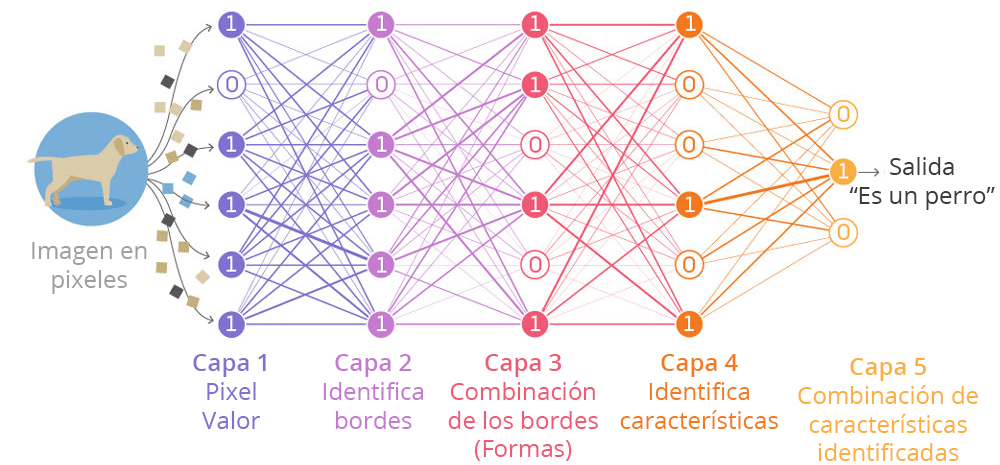
\includegraphics[width=\linewidth]{src/figures/deep_learning.png}
    \caption{Proceso de entrenamiento de una red deep learning \cite{deep_learning_img}}
    \label{fig:deep_learning_img}
\end{figure}

Entre los tipos de modelos de deep learning se encuentran 6 principales,
los cuales se explican de manera breve a excepción de las redes
neuronales convolucionales, las cuales son el enfoque principal del
presente trabajo de investigación.

\begin{itemize}
    \item \textbf{Redes Neuronales Convolucionales (CNN)}:
     utilizadas principalmente en el procesamiento de imágenes y 
     visión por computadora, conocidas por su capacidad para 
     capturar características espaciales.
    \item \textbf{Redes Neuronales Recurrentes (RNN)}: 
    diseñadas para trabajar con datos secuenciales, 
    como series temporales o lenguaje natural.
    \item \textbf{Redes Generativas Adversarias (GAN)}:
     compuestas de dos redes que compiten entre sí para generar datos
      sintéticos que se asemejan a datos reales, ampliamente utilizadas
       en generación de imágenes y contenido.
    \item \textbf{Autoencoders}: 
    redes que aprenden una representación comprimida de los datos
     de entrada y son útiles en tareas de reducción de dimensionalidad
      y compresión.
    \item \textbf{Modelos de difusión}: 
    Son modelos generativos entrenados con difusión directa e inversa
    para adicionar y eliminar ruido de las imágenes. estos modelos 
    generan datos en base a los datos de entrenamiento y añaden ruido 
    a los datos generados para aprender un proceso de eliminación de ruido.
    \item \textbf{Modelos de transformadores}: 
    Estos modelos usan una estructura de codificador y decodificador 
    para procesar texto. El codificador transforma el texto no procesado
    a representaciones llamadas incrustaciones, Después de esto,
    el decodificador usa esas incrustaciones resultantes 
    junto con palabras generadas previamente para generar texto que
    prediga la siguiente palabra en una oración de manera secuencial.
    \cite{ibm_deep_learning}
\end{itemize}

\subsection{Redes Neuronales Convolucionales}
Las redes neuronales convolucionales (CNN) son un tipo de red neuronal
que se utiliza principalmente en el procesamiento de imágenes y visión, 
aunque también son usadas en voz o audio. Estas redes neuronales se 
consituyen de varias capas las cuales pueden pertenecer a tres tipos:
capa convolucional, capa de agrupación y capa completamente conectada.
Para entender el funcionamiento de las redes neuronales convolucionales,
es necesario comprender el porque una imagen puede ser clasificada en
diferentes categorias; esto se debe a que las imagenes estan compuestas
por pixeles, los cuales son los elementos basicos de una imagen. Cada
pixel tiene un valor de intensidad que puede variar entre 0 y 255,
donde 0 representa el menor nivel de intensidad y 255 el mayor nivel
de intensidad.

\begin{figure}[ht!]
    \centering
    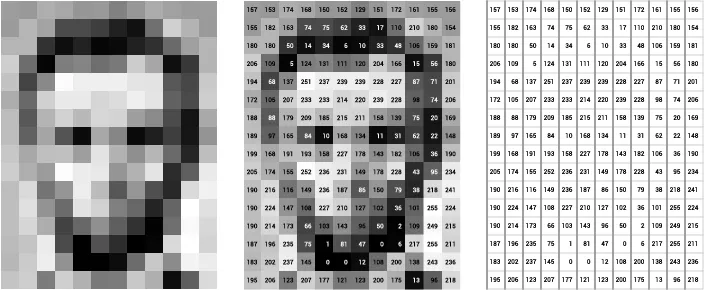
\includegraphics[width=\linewidth]{src/figures/grayscale_image.png}
    \caption{Imagen en escala de grises junto con sus valores por píxel \cite{grayscale_values}}
    \label{fig:grayscale_image}
\end{figure}

\newpage
Por otra parte, las imagenes pueden tener más de un canal
de color, como RGB (Red, Green, Blue), en este caso, cada canal de color
es una matriz de pixeles que representa un color en particular.

\begin{figure}[ht!]
    \centering
    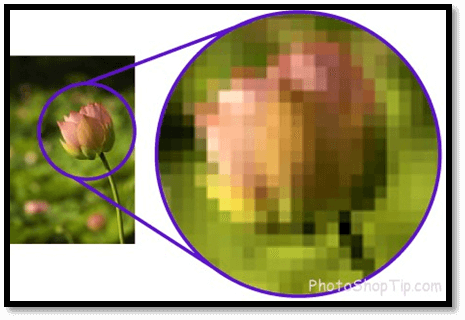
\includegraphics[width=\linewidth]{src/figures/pixels_in_image.png}
    \caption{Píxeles en una imagen \cite{pixels_in_image}}
    \label{fig:pixels_in_image}
\end{figure}

En adición, algunos conceptos básicos son definidos para asegurar la 
correcta comprensión de las redes neuronales convolucionales:

\begin{itemize}
    \item \textbf{Neurona}:
    Es la unidad básica de una red neuronal, la cual recibe una entrada
    y produce una salida al realizar una suma ponderada de sus conexiones
    a la que se le aplica una función de activación.
    \item \textbf{Función de activación}:
    Es una función matemática que se aplica a la salida de una neurona
    para determinar si esta se activa o no. Algunas de las funciones
    de activación más comunes son la función sigmoide, la función ReLU
    y la función tangente hiperbólica.
    \item \textbf{Capa de entrada}:
    Es la capa que recibe los datos de entrada, en esta, cada neurona
    corresponde a una de las características de entrada, como los pixeles
    de una imagen.
    Por ejemplo, si se tiene una imagen de 32x32 pixeles, la capa de
    entrada tendrá 1024 neuronas.
    \item \textbf{Capa oculta}:
    Son las posibles capas entre la capa de entrada y la capa de salida,
    las salidas de las neuronas de una capa oculta se convierten en las
    entradas de la siguiente capa.
    \item \textbf{Capa de salida}:
    Es la capa que produce la salida final de la red neuronal, en el caso
    de una red de clasificación, la capa de salida tendrá tantas neuronas
    como clases se desean clasificar.\cite{medium_cnn}
\end{itemize}


En cuanto a las funciones de activación, se explica el funcionamiento de 
cada una de ellas:

\begin{itemize}
    \item \textbf{Función Sigmoide}: 
    En algunos ejemplos es usada pero no es habitual, la función sigmoide
    se utiliza en la capa de salida de una red neuronal para problemas
    de clasificación binaria, ya que su salida se encuentra entre 0 y 1.
    Esto permite interpretar la salida como una probabilidad de pertenencia 
    a una clase específica. 
    Sin embargo, su uso ha disminuido en favor de otras funciones de activación,
     como ReLU, debido a problemas como el "desvanecimiento del gradiente" 
     y la saturación en valores extremos. A pesar de esto, la sigmoide sigue 
     siendo fundamental para entender cómo las redes neuronales pueden modelar
      relaciones no lineales y aprender patrones complejos \cite{sigmoid}.
    \begin{equation}
        f(x) = \frac{1}{1 + e^{-x}}
    \end{equation}

    \begin{figure}[H]
        \centering
        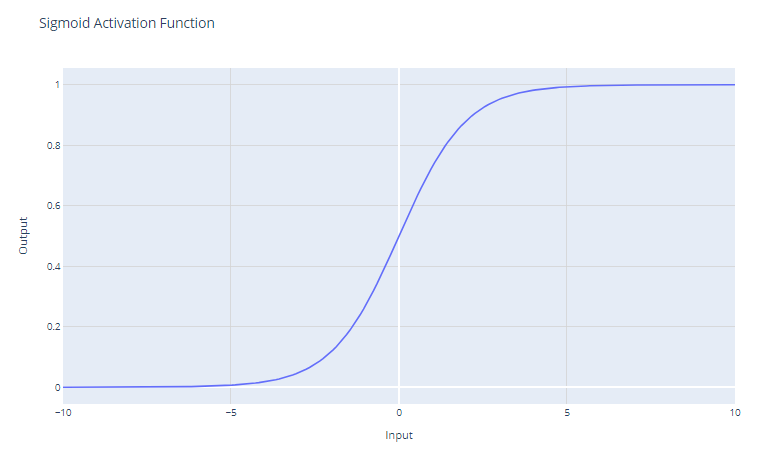
\includegraphics[width=\linewidth]{src/figures/sigmoid.png}
        \caption{Función Sigmoide \cite{sigmoid_graph}}
    \end{figure}

    \item \textbf{Función Tangente Hiperbólica}:
    La función de activación \textbf{tanh} (tangente hiperbólica) transforma valores 
    reales en un rango de -1 a 1, siendo útil en redes neuronales para centrar los 
    datos alrededor de cero. Su derivada es \(1 - \text{tanh}^2(x)\), lo que puede 
    causar saturación y desvanecimiento del gradiente en redes profundas. 
    A pesar de esto, es popular en capas ocultas por su capacidad de manejar tanto valores positivos 
    como negativos. \cite{activation_functions}

    \begin{equation}
        f(x) = \frac{e^{x} - e^{-x}}{e^{x} + e^{-x}}
    \end{equation}

    \begin{figure}[H]
        \centering
        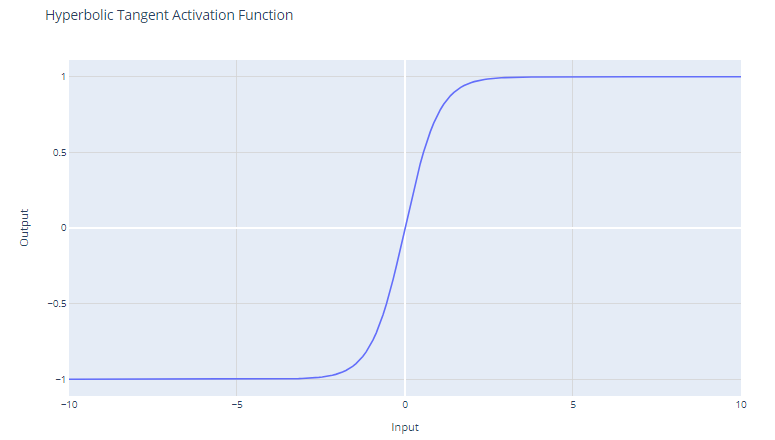
\includegraphics[width=\linewidth]{src/figures/tanh.png}
        \caption{Función Tangente Hiperbólica \cite{tanh_graph}}
    \end{figure}

    \item \textbf{Función ReLU (Rectified Linear Unit)}:
    La función de activación ReLU (Unidad Lineal Rectificada) es ampliamente utilizada 
    en redes neuronales por su simplicidad y efectividad, definida como:

        \[
        f(x) = \max(0, x)
        \]

    ReLU retorna 0 para valores negativos y el valor original para valores positivos, 
    permitiendo que el gradiente pase sin alteración en la retropropagación y evitando 
    el problema del gradiente que se desvanece. Aunque es lineal para entradas positivas, 
    su no linealidad en \( x = 0 \) le permite captar patrones complejos. 
    Además, su bajo costo computacional y tendencia a activaciones esparsas 
    favorecen la eficiencia en redes profundas. \cite{activation_functions}

    \begin{figure}[H]
        \centering
        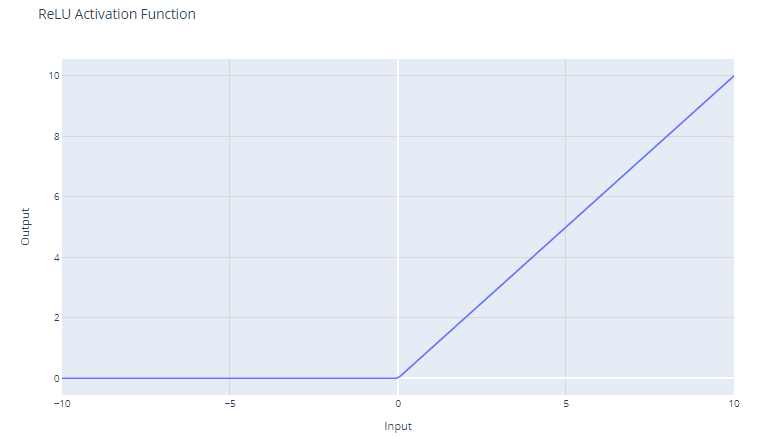
\includegraphics[width=\linewidth]{src/figures/relu.png}
        \caption{Función ReLU \cite{relu_graph}}
    \end{figure}

    \item \textbf{Función Softmax}:
    La función de activación Softmax es útil para clasificación multiclase, 
    convirtiendo un vector de entradas \( x_1, x_2, \dots, x_C \) en una distribución de probabilidad:

    \[
    f(x_i) = \frac{e^{x_i}}{\sum_{j} e^{x_j}}
    \]

    Cada salida representa la probabilidad de pertenencia a una clase, sumando a uno. 
    Softmax amplifica las diferencias entre entradas, haciendo que el valor más alto domine, 
    y se emplea comúnmente en la capa final de redes neuronales para tareas de clasificación 
    multiclase, proporcionando interpretaciones probabilísticas de confianza en las predicciones.
    \cite{activation_functions}

    \begin{figure}[H]
        \centering
        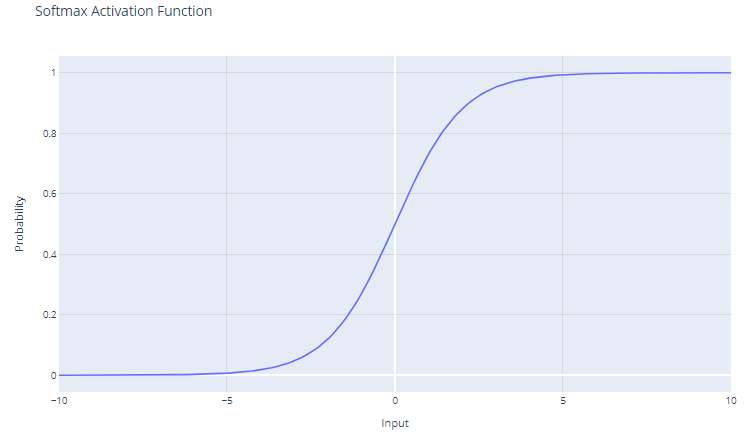
\includegraphics[width=\linewidth]{src/figures/softmax.png}
        \caption{Función Softmax \cite{softmax_graph}}
    \end{figure}
    
\end{itemize}

Una vez que se tienen claros los conceptos básicos, en las CNN se 
tienen tres tipos de capas, las cuales fueron descritas anteriormente:

\subsubsection{Capa Convolucional}

Esta capa es la parte fundamental de las redes neuronales convolucionales,
en esta capa son necesarios los elementos normales como las entradas, lo 
que la hace diferente es su necesidad de un filtro y un mapa de 
características. El filtro, también conocido como Kernel, es una matriz
de pesos (numeros) que se aplica a la imagen de entrada, este kernel se
desliza través de cada píxel para extraer características tales 
como bordes, texturas, formas, entre otros. La imagen resultante se
compone de un producto punto entre el kernel y cada pixel de la imagen. 
Los Kernel pueden ser de diferentes tamaños y pueden ser predefinidos 
o aprendidos durante el entrenamiento de la red.
Un ejemplo de un Kernel habitualmente usado es el Kernel de Sobel, el
cual se utiliza para detectar bordes en una imagen.

\begin{figure}[ht!]
    \centering
    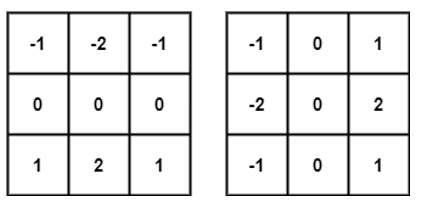
\includegraphics[width=\linewidth]{src/figures/sobel_kernel.png}
    \caption{Kernel de Sobel Horizontal y Vertical \cite{sobel_kernel}}
    \label{fig:sobel_kernel}
\end{figure}

Otro de los aspectos clave es que el tamaño del resultado se ve 
afectado por los siguientes hiperparametros:

\begin{itemize}
    \item \textbf{Cantidad de filtros}:
    La cantidad de filtros afecta a la profundidad de la salida, 
    esto porque cada filtro produce un mapa de características. 
    Por ejemplo, si se tienen 6 filtros y se recibe una imagen con 
    un solo canal de color, la salida tendrá 6 canales de color, pero
    si se recibe una imagen con 3 canales de color como RGB, la salida
    tendrá 18 canales de color (18 mapas de características).
    \item \textbf{Stride}:
    Es el número de píxeles que se desplaza el filtro en cada paso.
    \item \textbf{Padding}:
    Es la cantidad de píxeles que se añaden alrededor de la imagen, 
    generalmente se usa cuando el filtro es más grande que la imagen, 
    el borde que se le añade a la imagen es con valores de 0.
    \item \textbf{Tamaño del filtro}:
    Es el tamaño del filtro que se desliza sobre la imagen, generalmente
    se usan filtros de 3x3 o 5x5.
\end{itemize}

El calculo final para el tamaño que tendra un mapa de características
despues de aplicar un filtro a una imagen es el siguiente:

\begin{equation}
    \text{Salida} = \frac{N - K + 2P}{S} + 1
\end{equation}

Donde:
\begin{itemize}
    \item \textbf{N:} Tamaño de la imagen de entrada.
    \item \textbf{K:} Tamaño del filtro.
    \item \textbf{P:} Padding.
    \item \textbf{S:} Stride.
    \item \textbf{Salida:} Tamaño de la imagen de salida.
\end{itemize}

\newpage

Un ejemplo claro del calculo relizado con un filtro de 3x3 y una 
imagen de 5x5 es el siguiente:

\begin{figure}[ht!]
    \centering
    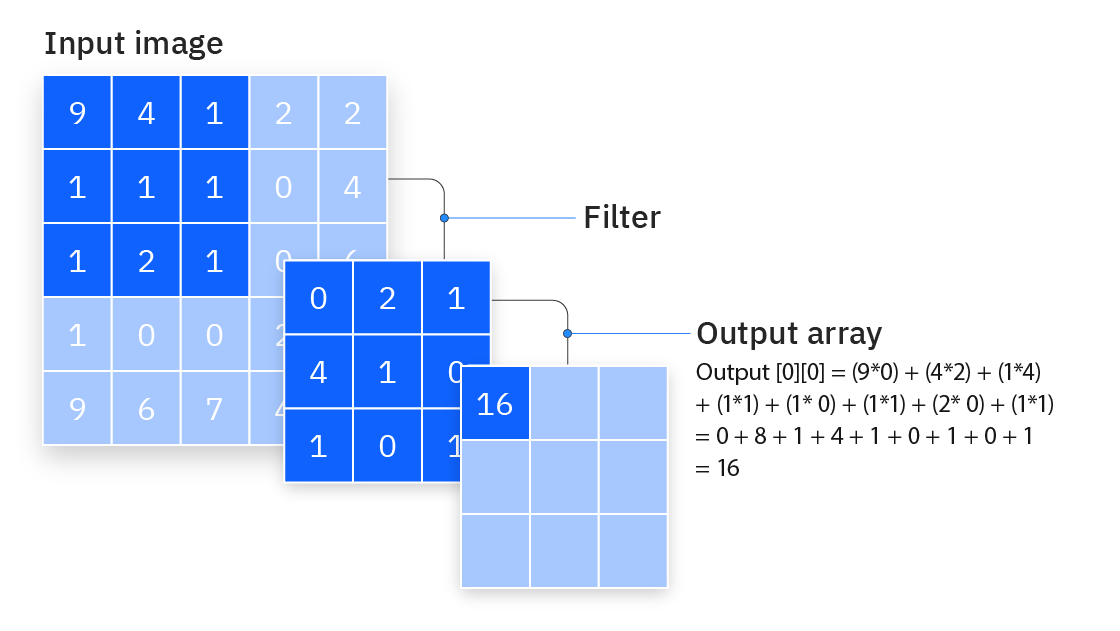
\includegraphics[width=\linewidth]{src/figures/kernel_calculation.png}
    \caption{Capa convolucional aplicada a una imagen \cite{kernel_calculation}}
    \label{fig:kernel_calculation}
\end{figure}

Cabe aclarar que puede haber más de una capa convolucional en una red,
esto convierte la estructura de la CNN en jerárquica, donde cada capa
que sigue a la anterior, aprende características más complejas.

\subsubsection{Capa de Agrupación}
La capa de agrupación (Pooling) es una capa que se utiliza para reducir
las dimensiones (Ancho y Alto) de la imagen, para disminuir el número
de parámetros y el costo computacional. La agrupacion aplica una función
de agregación a un conjunto de píxeles, como el promedio o el máximo; 
Esta capa aunque pierde información, ayuda a mejorar la generalización
de la red y su eficiencia. La capa de agrupacion puede ser de los 
siguientes tipos \cite{medium_pooling}:

\begin{itemize}
    \item \textbf{Max Pooling}:
    Se selecciona el valor máximo de un conjunto de píxeles, por lo tanto
    la salida despues de la capa de max pooling sera el mapa de características
    con los valores más altos.

    \begin{figure}[htbp]
        \centering
        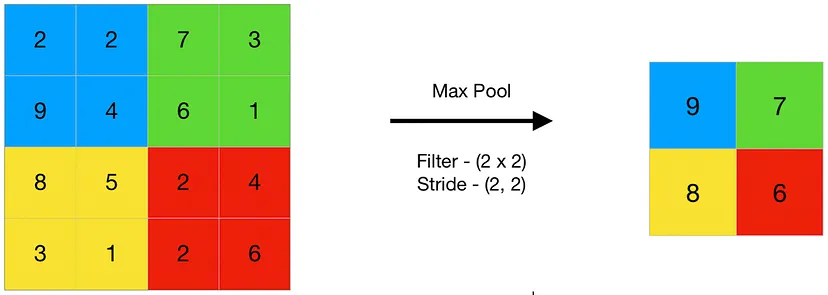
\includegraphics[width=0.8\linewidth]{src/figures/max_pooling.png}
        \caption{Max Pooling aplicado a un mapa de características \cite{max_pooling}}
        \label{fig:max_pooling}
    \end{figure}

    \item \textbf{Average Pooling}:
    Se calcula el promedio de un conjunto de píxeles en el mapa de características,
    por lo tanto la salida despues de la capa de average pooling sera el mapa de
    características con los valores promedio.

    \begin{figure}[htbp]
        \centering
        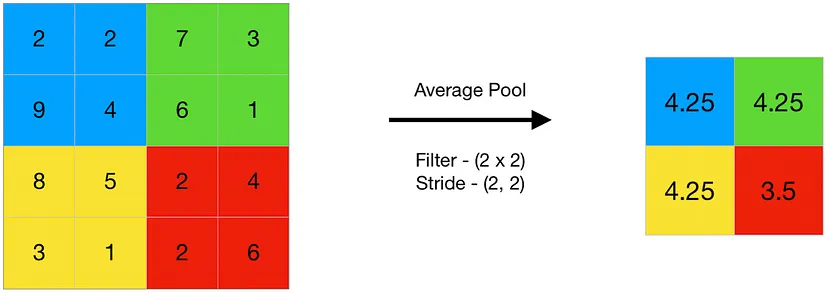
\includegraphics[width=0.8\linewidth]{src/figures/average_pooling.png}
        \caption{Average Pooling aplicado a un mapa de características \cite{average_pooling}}
        \label{fig:average_pooling}
    \end{figure}
\end{itemize}

Además de estos tipos, tambien hay agrupamiento global, el cual calcula
el promedio o el máximo de cada canal de características, en lugar de
hacerlo por regiones; Esto da como salida un solo valor por canal de
características.

\subsubsection{Capa Completamente Conectada}
Normalmente, suele haber una capa entre la capa de agrupación y la capa
completamente conectada, esta capa se conoce como capa de aplanamiento
(Flatten), la cual convierte la matriz de características en un vector
unidimensional, para que pueda ser procesado por la capa completamente
conectada.

\begin{figure}[htbp]
    \centering
    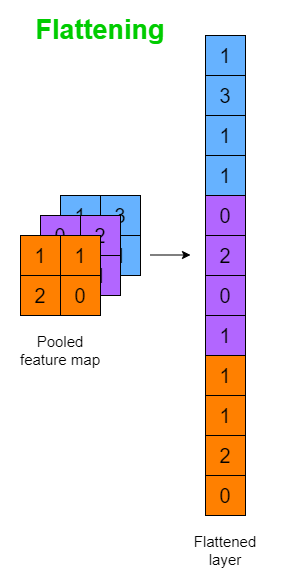
\includegraphics[width=0.45\linewidth]{src/figures/flatten.png}
    \caption{Capa de aplanamiento aplicada a tres mapas de características \cite{capa_aplanada}}
    \label{fig:flatten}
\end{figure}

Por último, la capas capas completamente conectadas son las capas
de una RNA tradicional, donde cada neurona de la capa está conectada
con todas las neuronas de la capa anterior. Estas capas se utilizan
para clasificar las características extraídas por las capas convolucionales
y de agrupación. La capa completamente conectada se encarga de realizar
la clasificación final de la red, en donde se obtiene la probabilidad
de que una imagen pertenezca a una clase en particular mediante la 
función de activación softmax.

\begin{figure}[htbp]
    \centering
    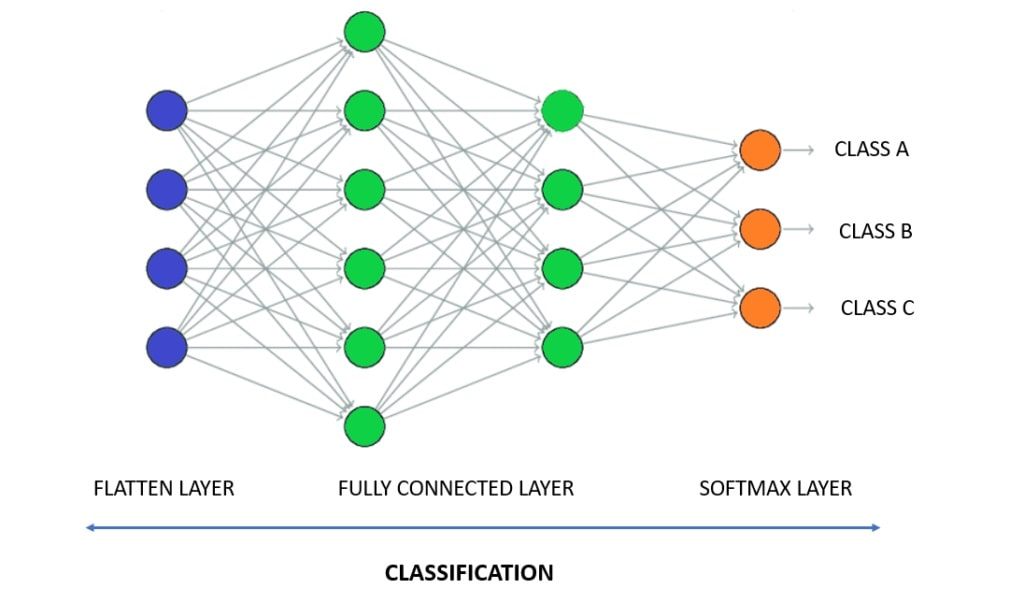
\includegraphics[width=0.9\linewidth]{src/figures/fully_connected_layer.png}
    \caption{Capa completamente conectada \cite{capa_conectada}}
    \label{fig:fully_connected}
\end{figure}


\subsection{LeNet}

\subsubsection{Historia}

La historia de LeNet refleja un progreso innovador en el desarrollo 
de redes neuronales convolucionales aplicadas a la identificación de 
patrones visuales. En 1988, Yann LeCun se unió al Departamento de 
Investigación de Sistemas Adaptativos en AT\&T Bell Labs, dirigido 
por Lawrence D. Jackel. Desde entonces, LeCun y su equipo comenzaron 
a trabajar en modelos que pudieran reconocer caracteres manuscritos 
de manera eficiente, en particular códigos postales.

En 1989, publicaron la primera versión de una red neural convolucional
 (LeNet-1) diseñada específicamente para leer dígitos manuscritos. 
 Esta versión utilizaba núcleos de convolución fijos y se entrenaba
 mediante el algoritmo de retropropagación, lo cual era una innovación 
 importante en el campo. Este primer modelo mostró que la combinación 
 de redes convolucionales y retropropagación podía aprender a 
 generalizar características visuales relevantes con una alta precisión,
  incluso en tareas complejas como el reconocimiento de dígitos 
  manuscritos proporcionados por el Servicio Postal de los Estados 
  Unidos. En este año también, LeCun demostró que la restricción 
  del número de parámetros libres mejoraba significativamente la 
  capacidad de generalización del modelo.

En 1990, se publicaron más investigaciones sobre la aplicación de redes 
de retropropagación para reconocimiento de caracteres, logrando un 
margen de error bajo en la identificación de números en imágenes, 
con una tasa de rechazo controlada. Estos resultados alentaron 
investigaciones continuas, y en 1994, LeCun y su equipo desarrollaron 
la base de datos MNIST, diseñada como un estándar para evaluar redes 
de reconocimiento de dígitos. LeNet-4 se entrenó para abordar el tamaño 
y la complejidad de esta base de datos.

El esfuerzo culminó en 1995 con el desarrollo de LeNet-5, 
una arquitectura más avanzada que integraba métodos adicionales 
para mejorar la precisión en la clasificación de caracteres manuscritos. 
Este modelo no solo superó otros métodos en pruebas de referencia, 
sino que también fue aplicado en sistemas de lectura automática de 
millones de cheques bancarios al día. En 1998, LeCun y su equipo 
presentaron estos avances como ejemplos de aplicaciones prácticas en el 
reconocimiento de caracteres manuscritos.

Aunque las redes neuronales modernas han evolucionado significativamente 
desde LeNet, esta serie de modelos sentó las bases para el diseño de 
arquitecturas convolucionales complejas, marcando un hito en la historia 
de la inteligencia artificial y el aprendizaje profundo \cite{lenet_history_geeks} \cite{lenet_neha}.

\subsubsection{versiones}

\begin{itemize}
    \item \textbf{LeNet-1}: 
    LeNet-1 fue uno de los primeros modelos de redes neuronales 
    convolucionales diseñado por Yann LeCun y su equipo. 
    La arquitectura estaba enfocada en reconocer dígitos manuscritos 
    y se basaba en la aplicación de capas de convolución y capas de 
    subsampling o pooling. Los detalles de su arquitectura son los 
    siguientes:

    \begin{figure}[htbp]
        \centering
        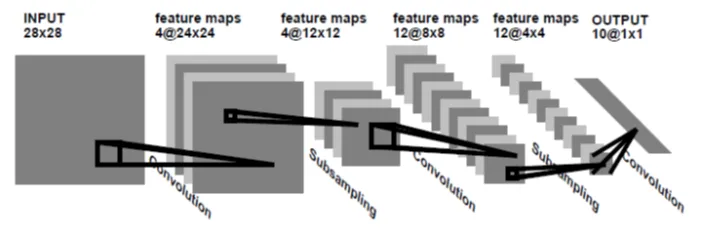
\includegraphics[width=\linewidth]{src/figures/lenet_1.png}
        \caption{Arquitectura de LeNet-1 \cite{Lenet_1}}
        \label{fig:lenet-1}
    \end{figure}

    \textbf{Entrada}: Imagen de 28x28 píxeles en escala de grises.  
    \textbf{Capa de convolución 1}: genera cuatro mapas de características
    de 24x24 píxeles mediante la convolución con kernels predefinidos de 5x5 píxeles.

    \textbf{Capa Average Pooling 1}: reduce la dimensión de los mapas de características
    a 12x12 píxeles usando una ventana de 2x2 píxeles para calcular el promedio.

    \textbf{Capa de convolución 2}: produce 12 mapas de características 
    de 8x8 píxeles mediante la convolución con kernels de 5x5 píxeles.

    \textbf{Capa Average Pooling 2}: reduce la dimensión de los mapas de 
    características a 4x4 píxeles usando una ventana de 2x2 píxeles 
    para calcular el promedio.

    \textbf{Capa de Salida}: capa completamente conectada con 10 neuronas
    para clasificar los dígitos del 0 al 9.

    \item \textbf{LeNet-4}:
    
    LeNet-4 es una versión mejorada de LeNet-1, diseñada para manejar 
    imágenes de entrada ligeramente más grandes y con más capacidad 
    de aprendizaje. La arquitectura de LeNet-4 tiene los siguientes 
    componentes:

    \begin{figure}[htbp]
        \centering
        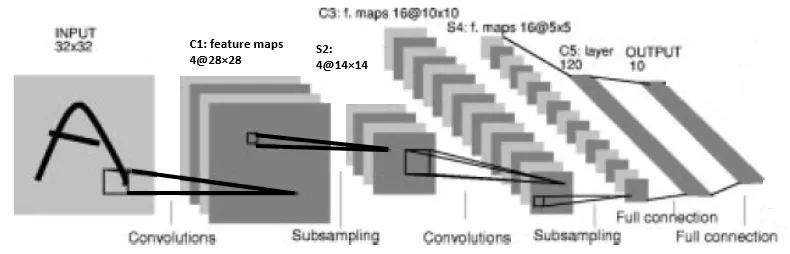
\includegraphics[width=\linewidth]{src/figures/lenet_4.png}
        \caption{Arquitectura de LeNet-4 \cite{Lenet_4}}
        \label{fig:lenet-4}
    \end{figure}

    \textbf{Entrada}: Imagen de 32x32 píxeles en escala de grises.

    \textbf{Capa de convolución 1}: genera cuatro mapas de 
    características de 28x28 píxeles mediante la convolución con
    kernels de 5x5 píxeles.

    \textbf{Capa Average Pooling 1}: reduce la dimensión de los mapas
    de características a 14x14 píxeles usando una ventana de 2x2 píxeles
    para calcular el promedio.

    \textbf{Capa de convolución 2}: produce 16 mapas de características
    de 10x10 píxeles mediante la convolución con kernels de 5x5 píxeles.

    \textbf{Capa Average Pooling 2}: reduce la dimensión de los mapas
    de características a 5x5 píxeles usando una ventana de 2x2 píxeles
    para calcular el promedio. 

    \textbf{Flatten Layer}: convierte los mapas de características en
    un vector unidimensional.

    \textbf{Capa completamente conectada 1}: 120 neuronas con función
    de activación sigmoidal o tangente hiperbólica.

    \textbf{Capa de Salida}: 10 neuronas con función
    de activación softmax para clasificar los dígitos del 0 al 9.

    \item \textbf{LeNet-5}:

    LeNet-5 es la versión más popular de la arquitectura LeNet, 
    introducida en 1995. Es similar a LeNet-4, pero incluye algunos 
    ajustes adicionales en la cantidad de neuronas y conexiones. 
    Su estructura es la siguiente:

    \begin{figure}[ht!]
        \centering
        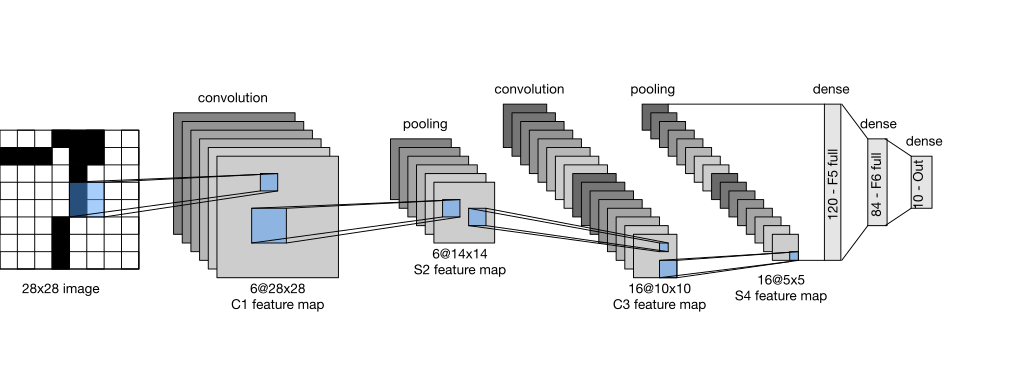
\includegraphics[width=\linewidth]{src/figures/lenet_5.png}
        \caption{Arquitectura de LeNet-5 \cite{Lenet_5}}
        \label{fig:lenet-5}
    \end{figure}

    \textbf{Entrada}: Imagen de 32x32 píxeles en escala de grises.

    \textbf{Capa de convolución 1}: genera seis mapas de características
    de 28x28 píxeles mediante la convolución con kernels de 5x5 píxeles.

    \textbf{Capa Average Pooling 1}: reduce la dimensión de los mapas
    de características a 14x14 píxeles usando una ventana de 2x2 píxeles
    para calcular el promedio.

    \textbf{Capa de convolución 2}: produce 16 mapas de características
    de 10x10 píxeles mediante la convolución con kernels de 5x5 píxeles.

    \textbf{Capa Average Pooling 2}: reduce la dimensión de los mapas
    de características a 5x5 píxeles usando una ventana de 2x2 píxeles
    para calcular el promedio.

    \textbf{Flatten Layer}: convierte los mapas de características en
    un vector unidimensional.

    \textbf{Capa completamente conectada 1}: 120 neuronas con función
    de activación sigmoidal o tangente hiperbólica.

    \textbf{Capa completamente conectada 2}: 84 neuronas con función
    de activación sigmoidal o tangente hiperbólica.

    \textbf{Capa de Salida}: 10 neuronas con función
    de activación softmax para clasificar los dígitos del 0 al 9.

    \space

    \item \textbf{Boosted LeNet-4}:
    
    \begin{figure}[htbp]
        \centering
        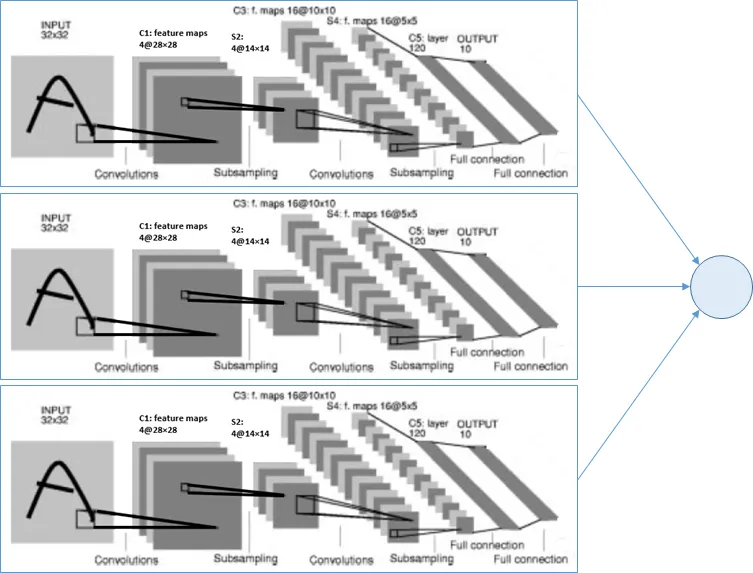
\includegraphics[width=\linewidth]{src/figures/lenet_4_boosted.png}
        \caption{Arquitectura de Boosted LeNet-4 \cite{LeNet_4_boosted}}
        \label{fig:boosted_lenet_4}
    \end{figure}

    En una versión mejorada llamada Boosted LeNet-4, se implementó 
    una técnica de combinación de múltiples redes para aumentar 
    la precisión de LeNet-4. Esta técnica de boosting combinaba los 
    resultados de tres redes LeNet-4; se sumaban las salidas y el 
    valor más alto era la clase predicha. Además, si una red obtenía 
    una salida con alta confianza, las demás redes no se usaban. 
    Con esta modificación, Boosted LeNet-4 redujo la tasa de error 
    a 0.7\%, mejorando incluso a LeNet-5.

\end{itemize}

\subsubsection{Aplicaciones}

La red neuronal convolucional LeNet ha demostrado ser una 
arquitectura fundamental que trasciende su propósito inicial 
de reconocimiento de dígitos manuscritos tal como se ve presente
en el desarrolló realizado por Yann LeCun en su articulo sobre LeNet,
en aquella ocación la implementación logro una precisión de 
clasificación de aproximadamente el 99,2\%, aunque el documento 
original es largo y trata varios temas, cabe recalcar la comparación
con modelos de clasificación del momento dando un porcentaje de 
error bastante más bajo con respecto a los otros modelos, entre los
modelos contra los cuales fue comparado están: K-NN, Support Vector
Machine y diferentes combinaciones de capas de neuronas. 

\begin{figure}[htbp]
    \centering
    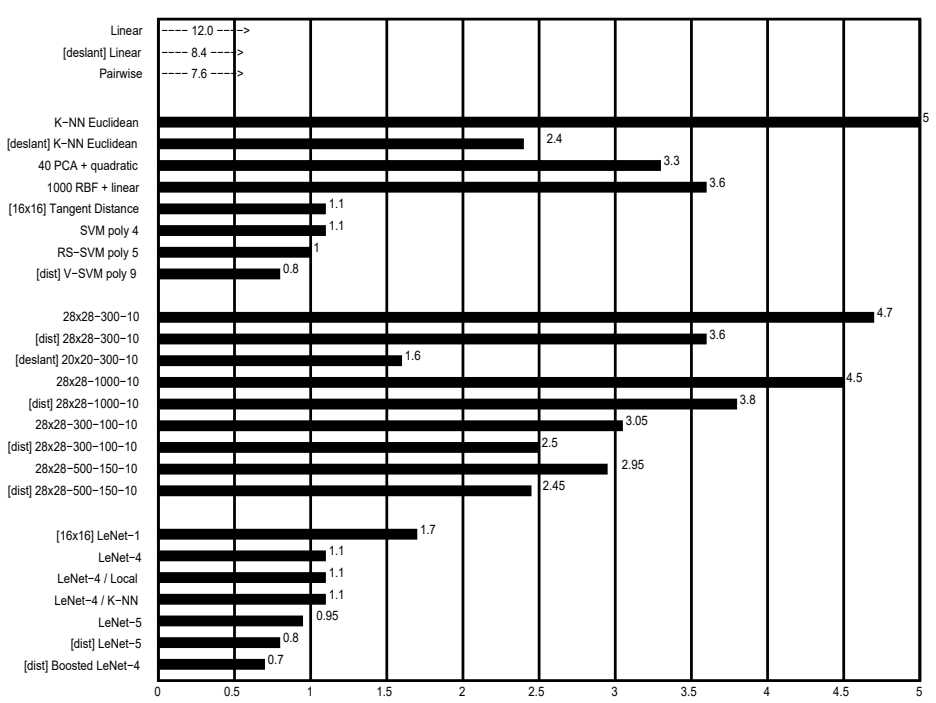
\includegraphics[width=\linewidth]{src/figures/lenet_comparison.png}
    \caption{Comparación de LeNet con otros modelos de clasificación \cite{lecun_comparison_image}}
    \label{fig:lenet_comparison}
\end{figure}

Sus aplicaciones se han diversificado significativamente en diversos 
campos tecnológicos y científicos. En el sector de procesamiento documental, 
 esta arquitectura facilita la automatización de tareas de gestión y 
 clasificación de documentos, mientras que en el ámbito médico 
 contribuye al análisis de imágenes diagnósticas para la identificación 
 de anomalías, un claro ejemplo de esto es el articulo llamado 
 A Modified LeNet CNN for Breast Cancer Diagnosis in Ultrasound Images 
 \cite{lenet_medical} donde se utiliza una versión modificada de LeNet
    para la detección de cancer de mama en imagenes de ultrasonido, 
 este modelo se planteó como un clasificador de tumores benignos y
    malignos, obteniendo una precisión del 89.91\% en el reconocimiento
    de imagen. El sistema también ha revolucionado los procesos de 
 autenticación biométrica mediante el análisis de firmas y huellas 
 dactilares, fortaleciendo los protocolos de seguridad. 
 En el contexto del análisis de video en tiempo real, los principios 
 de LeNet han sido instrumentales para el desarrollo de sistemas de 
 vigilancia y reconocimiento facial, En este campo, se tiene como 
 ejemplo práctico el artículo online publicado por Andrii Gozhulovskyi
 llamado Classification of Traffic Signs with LeNet-5 CNN
 \cite{lenet_traffic_sings} donde se usan los datos de las señales de 
 trafico alemanas para entrenar una red LeNet-5 que permita 
 clasificarlas, este articulo comprende un tutorial paso a paso de 
 como implementar la red junto con sus datos, evaluacion y graficación
 de resultados y métricas. Adicionalmente, su implementación 
 en el reconocimiento de caracteres manuscritos ha facilitado la
  digitalización de documentos históricos y el procesamiento 
  automatizado de formularios en diversos sectores, incluyendo servicios
   postales y bancarios. La versatilidad de esta arquitectura ha 
   permitido su adaptación para la clasificación de objetos en entornos 
   industriales y comerciales, demostrando su valor en sistemas de 
   control de calidad y gestión de inventarios 
   \cite{lenet_history_geeks}.

\subsubsection{Limitaciones}

Con respecto a las limitaciones de la red LeNet, se pueden mencionar
algunas de las siguientes:

\begin{itemize}
    \item \textbf{Capacidad de generalización}:
    Al ser una arquitectura relativamente simple, LeNet puede tener
    una limitacion para generalizar tareas complejas, esto debido a su
    pequeño tamaño y cantidad de capas.
    \item \textbf{Tamaño de entrada}:
    Se restringe su aplicabilidad a imagenes de tamaño fijo (32x32),
    lo cual es ineficaz para aplicaciones del mundo real donde 
    las imagenes varian en tamaño.
    \item \textbf{Falta de escalabilidad}:
    Puede ser un modelo que se queda corto en adaptaciones a 
    datos modernos y demandas de deep learning.\cite{lenet_neha}
\end{itemize}